\section{طراحی فیزیکی و تخمین مساحت}
\label{sec:book-physical-design}
\subsection{\lr{Floorplan} و بازخورد به معماری}
\lr{Physical Design} جای سلول‌ها، سیم‌ها، اتصال‌های تغذیه و هندسه لایه‌های تراشه
را تعیین می‌کند. \lr{Floorplan} تخمین اولیه ابعاد بلوک‌های بزرگ و موقعیت نسبی آن‌هاست.
این طرح برای ارزیابی جاگرفتن مدار، طول اتصال‌ها و \lr{Routing Congestion} به کار می‌رود.
تراکم مسیر به وضعیتی اشاره دارد که تقاضای سیم‌کشی در ناحیه‌ای به ظرفیت مسیرهای
موجود نزدیک شود یا از آن بیشتر شود \cite[بخش \secnum{۱.۱۰.۱}]{weste}.

تخمین مکان بلوک‌ها با تصمیم‌های \lr{Microarchitecture} ارتباط دوطرفه دارد.
در مثال مفهومی کتاب، نزدیک‌شدن \lr{Cache} به واحد اجرا ممکن است زمان دسترسی را
از دو دوره به یک دوره کاهش دهد. این تغییر می‌تواند انتخاب ظرفیت \lr{Cache} و
سپس \lr{Floorplan} را تغییر دهد. چنین نتیجه‌ای نیازمند تأیید زمان‌بندی طراحی واقعی است.
طرح اولیه باید با دقیق‌شدن منطق، اندازه سلول‌ها و سیم‌کشی بازبینی شود.

در مثال \lr{MIPS} کتاب، \lr{Controller}، \lr{Datapath}، کانال سیم‌کشی و
\lr{Pad Frame} بلوک‌های اصلی‌اند. \lr{Pad} محل اتصال الکتریکی سطح تراشه به محیط
بیرون است. از ۴۰ \lr{Pad}، تعداد ۲۹ برای سیگنال و ۱۱ برای تغذیه و زمین هستند.
شکل \ref{fig:impl-floorplan} ابعاد اصلی شکل \secnum{۱.۶۲} کتاب را بازنمایی می‌کند.

\begin{figure}[ht]
\centering
\begin{latin}
\PersianMathDigits
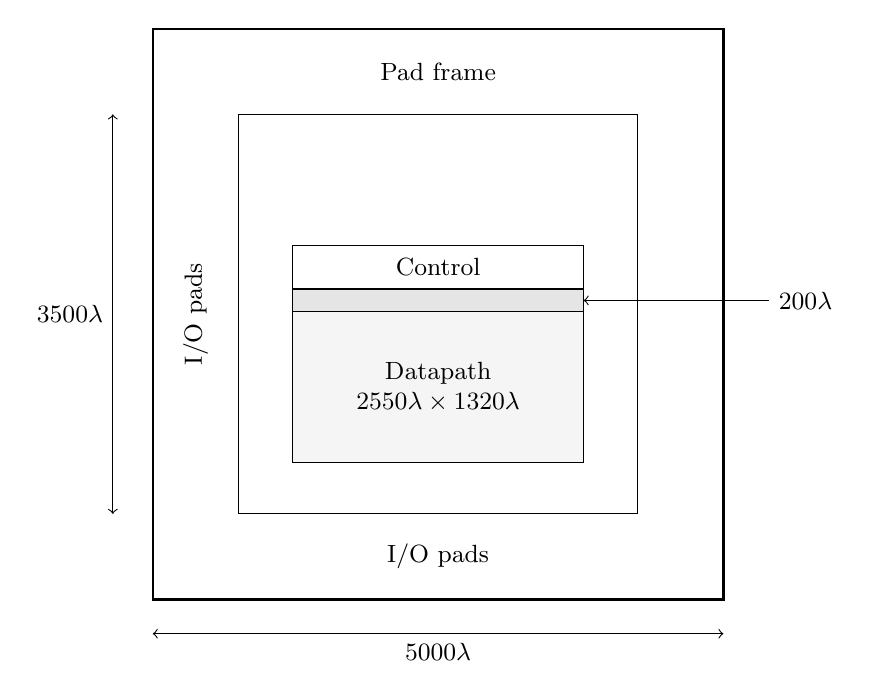
\begin{tikzpicture}[x=0.00145cm,y=0.00145cm,font=\small]
\draw[thick] (0,0) rectangle (5000,5000);
\draw (750,750) rectangle (4250,4250);
\node at (2500,4625) {Pad frame};
\node[rotate=90] at (375,2500) {I/O pads};
\node at (2500,375) {I/O pads};
\draw[fill=gray!8] (1225,1200) rectangle (3775,2520);
\node[align=center] at (2500,1860) {Datapath\\$2550\lambda\times1320\lambda$};
\draw[fill=gray!20] (1225,2520) rectangle (3775,2720);
\draw (1225,2720) rectangle (3775,3100);
\node at (2500,2910) {Control};
\draw[<-] (3775,2620)--(5400,2620) node[right] {$200\lambda$};
\draw[<->] (0,-300)--(5000,-300) node[midway,below] {$5000\lambda$};
\draw[<->] (-350,750)--(-350,4250) node[midway,left] {$3500\lambda$};
\end{tikzpicture}
\end{latin}
\caption{\lr{Floorplan} آموزشی با نسبت ابعاد اصلی کتاب. مستطیل میانی، فضای قابل‌استفاده
داخل \lr{Pad Frame} است. نوار خاکستری کانال کنترل را نشان می‌دهد. جزئیات تک‌تک \lr{Pad}ها حذف شده‌اند
\cite[شکل \secnum{۱.۶۲}]{weste}.}
\label{fig:impl-floorplan}
\end{figure}

\subsection{تبدیل طول و مساحت در مثال کتاب}
در فناوری آموزشی \qty{0.6}{\micro\metre} این مثال، \(\lambda=\qty{0.3}{\micro\metre}\)
است. بنابراین ضلع \(5000\lambda\) برابر \qty{1500}{\micro\metre} یا
\qty{1.5}{\milli\metre} می‌شود. رابطه عمومی تبدیل مساحت چنین است
\begin{equation}
 A_{\mathrm{physical}}=A_{\lambda}\lambda^2.
 \label{eq:impl-area-conversion}
\end{equation}
در این رابطه \(A_{\lambda}\) مقدار عددی مساحت در واحد \(\lambda^2\) است.
چون هر دو بعد طول در \(\lambda\) ضرب می‌شوند، ضریب تبدیل مساحت مربع می‌شود.
در این فناوری، \(1\lambda^2=\qty{0.09}{\micro\metre\squared}\) است.

ابعاد هر \lr{Pad} در کتاب \(750\lambda\times350\lambda\) ذکر شده‌اند.
با کنارگذاشتن حاشیه شعاعی \(750\lambda\) در هر طرف، ضلع فضای داخلی
\(5000-2(750)=3500\lambda\) می‌شود. پس
\begin{align}
 A_{\mathrm{die}}&=(5000\lambda)^2
 =25\times10^6\lambda^2=\qty{2.25}{\milli\metre\squared},\notag\\
 A_{\mathrm{inside}}&=(3500\lambda)^2
 =12.25\times10^6\lambda^2=\qty{1.1025}{\milli\metre\squared}.
 \label{eq:impl-die-core}
\end{align}
مساحت داخل قاب، ظرفیت هندسی موجود را بیان می‌کند. ابعاد بسته پردازنده، شامل دو
بلوک و کانال میان آن‌ها، کوچک‌تر است. با ابعاد گرد‌شده \lr{Floorplan} داریم
\begin{align}
 H_{\mathrm{core}}&=(1320+200+380)\lambda=1900\lambda,\notag\\
 A_{\mathrm{core}}&=(2550)(1900)\lambda^2
 =4.845\times10^6\lambda^2\approx4.8\times10^6\lambda^2.
 \label{eq:impl-core-area}
\end{align}
سهم \lr{Datapath}، کنترل و کانال به‌ترتیب
\(3.366\times10^6\lambda^2\)، \(0.969\times10^6\lambda^2\) و
\(0.510\times10^6\lambda^2\) است. جمع آن‌ها دقیقاً مقدار
\eqref{eq:impl-core-area} را می‌دهد. مقدار فیزیکی متناظر \qty{0.43605}{\milli\metre\squared}
است که برای گزارش تقریبی می‌توان \qty{0.44}{\milli\metre\squared} نوشت.

در این مثال، فضای موردنیاز \lr{Pad Frame} اندازه \lr{Die} را تعیین می‌کند و طراحی
\lr{Pad-limited} است. در طراحی \lr{Core-limited}، اندازه منطق داخلی عامل تعیین‌کننده
مساحت است. کاهش یک بلوک داخلی در حالت اول، تا زمانی که نیاز قاب ثابت بماند،
الزاماً اندازه نهایی \lr{Die} را کاهش نمی‌دهد \cite[صفحه ۴۷]{weste}.

\subsection{گونه‌های ساختار و \lr{Standard Cell}}
کتاب ساختارهای روی تراشه را در گروه‌های \lr{Random Logic}، \lr{Datapath}،
\lr{Array}، \lr{Analog} و \lr{I/O} توضیح می‌دهد \cite[صفحه ۴۸]{weste}.
\lr{Random Logic} اتصال‌های کم‌نظم، مانند \lr{Decoder} منطقی عمومی، دارد.
در \lr{Datapath}، کار مشابه در چند بیت تکرار می‌شود. در \lr{Array}، سلول‌های مشابه
در دو بعد تکرار می‌شوند، مانند \lr{RAM}، \lr{ROM} و \lr{PLA}.
مدار \lr{Analog} و سلول \lr{I/O} به نیازهای الکتریکی و فناوری ویژه خود وابسته‌اند.
تکرار سلولِ طراحی و بررسی‌شده، هزینه طراحی آرایه‌ها را میان نمونه‌های متعدد تقسیم می‌کند.

\lr{Standard Cell} یک سلول کتابخانه‌ای با تابع و هندسه ازپیش‌تعریف‌شده، مانند
\lr{Inverter}، \lr{NAND} یا \lr{Flip-flop}، است. در نمونه کتاب، ریل‌های افقی
تغذیه در \lr{Metal1} عرض \(8\lambda\) و فاصله مرکز تا مرکز \(90\lambda\) دارند.
\lr{nMOS}ها در ناحیه پایین \(40\lambda\) و \lr{pMOS}ها در ناحیه بالای
\(50\lambda\) قرار می‌گیرند. هم‌ترازی ریل و \lr{n-well} امکان اتصال سلول‌های مجاور
از طریق \lr{Abutment} را فراهم می‌کند.

عرض سلول مضربی از \(8\lambda\) است تا تعداد صحیحی مسیر عمودی \lr{Metal2}
داشته باشد. ورودی و خروجی در \lr{Metal2} در دسترس‌اند. \lr{Poly} عمدتاً عمودی و
\lr{Diffusion} و \lr{Metal1} عمدتاً افقی‌اند. اتصال‌های \lr{Substrate} و
\lr{Well} زیر ریل‌ها جا می‌گیرند. فاصله تکرار ردیف‌ها حداقل \(110\lambda\) است.
این اعداد، قواعد کتابخانه آموزشی همان مثال هستند \cite[بخش \secnum{۱.۱۰.۲}]{weste}.

در فرآیند دوفلزی، مسیرهای افقی میان ردیف‌ها به کانال نیاز دارند و تعداد سیم‌ها
ارتفاع کانال را تعیین می‌کند. در مثال سه‌فلزی، \lr{Metal3} افقی با
\lr{Pitch} برابر \(10\lambda\)، روی ارتفاع \(110\lambda\) حدود ۱۱ مسیر فراهم می‌کند.
اگر تقاضای سیم‌کشی در این ظرفیت جا بگیرد، کانال جداگانه می‌تواند حذف شود.
در مثال \lr{MIPS}، جهت‌های غالب \lr{Metal1}، \lr{Metal2} و \lr{Metal3}
به‌ترتیب افقی، عمودی و افقی‌اند. این ترتیب عبور سیم‌ها در لایه‌های مختلف را آسان می‌کند.

کتاب در شکل‌های \secnum{۱.۶۴} و \secnum{۱.۶۵}، نتیجه \lr{Place and Route}
کنترل‌کننده و پردازنده را نشان می‌دهد. نمونه پردازنده در فناوری \qty{130}{\nano\metre}
با هفت لایه فلز، ۲۶ ردیف سلول و حدود \(4\times10^6\lambda^2\) مساحت دارد.
مقایسه تلاش طراحی و سرعت در متن کتاب مربوط به همین زمینه تاریخی است.

\subsection{\lr{Pitch Matching} و \lr{Slice Plan}}
\lr{Pitch} فاصله تکرار یک ساختار است. برای سلول‌هایی که در امتداد یک لبه به هم
می‌چسبند، اندازه و محل اتصال‌های آن لبه باید هماهنگ شوند. این هماهنگی
\lr{Pitch Matching} نام دارد. کوچک‌کردن یک سلول هنگامی که ابعاد نهایی را سلول
همسایه تعیین می‌کند، ممکن است تنها فضای خالی ایجاد کند. بزرگ‌کردن همان سلول نیز
می‌تواند ابعاد همسایه و کل آرایه را افزایش دهد \cite[شکل \secnum{۱.۶۶}]{weste}.

برای نمونه فرضی، چهار سلول با عرض \(w_A\) کنار هم به بلوکی با عرض \(w_B\)
متصل می‌شوند. اگر لبه‌های بیرونی باید هم‌تراز بمانند، عرض موردنیاز ناحیه
\(W=\max(4w_A,w_B)\) است. با \(w_A=20\lambda\) و \(w_B=90\lambda\)،
عرض \(90\lambda\) می‌شود. کاهش \(w_A\) به \(18\lambda\) همچنان همان عرض
نهایی را می‌دهد. برای استفاده از فضای آزاد باید سازمان‌دهی ناحیه نیز بازنگری شود.

\lr{Slice Plan} ترتیب \lr{Wordslice}ها و تخصیص مسیرها در هر \lr{Bitslice} را
پیش از رسم جزئیات مشخص می‌کند. در شکل \secnum{۱.۶۸} کتاب، نقطه روی مسیر بیان می‌کند
که گذرگاه علاوه بر عبور از سلول، در آن سلول مصرف یا تولید می‌شود. پهنای هر جزء با
تعداد مسیر نوشته شده است. بیشترین تراکم این مثال روی \lr{Register File} و برابر
هفت مسیر است \cite[بخش \secnum{۱.۱۰.۴}]{weste}.

جمع عرض اجزای شکل کتاب ۳۱۹ مسیر است. با \lr{Pitch} برابر \(8\lambda\)،
عرض \lr{Datapath} چنین محاسبه می‌شود
\begin{equation}
 W_{\mathrm{data}}=319\times8\lambda=2552\lambda.
 \label{eq:impl-slice-width}
\end{equation}
عدد \(2550\lambda\) در \lr{Floorplan}، مقدار گرد‌شده همین تخمین است.
ارتفاع از هشت \lr{Bitslice}، یک ردیف \lr{Zipper} و سه ردیف \lr{Address Decoder}
ساخته می‌شود. پس با ۱۲ ردیف و فاصله \(110\lambda\)، ارتفاع
\(12(110)\lambda=1320\lambda\) است. فضای خالی ردیف‌های \lr{Decoder} در طراحی
فشرده‌تر می‌تواند برای بخش دیگری مانند کنترل استفاده شود. این تغییر به سازگاری
اتصال و زمان‌بندی نیاز دارد.

\subsection{\lr{Array} و نمونه \lr{PLA}}
\lr{Programmable Logic Array} یا \lr{PLA} توابع به صورت \lr{Sum of Products}
را با دو صفحه پیاده می‌کند. \lr{AND Plane} جمله‌های حاصل‌ضرب و \lr{OR Plane}
ترکیب آن‌ها را می‌سازد. برای نمونه، \(F=ab+ac\) به دو جمله حاصل‌ضرب و یک خروجی
نیاز دارد. در کنترل‌کننده کتاب، این ساختار منطق حالت بعد و خروجی \lr{FSM} را
پیاده می‌کند \cite[بخش \secnum{۱.۱۰.۵}، شکل \secnum{۱.۶۹}]{weste}.

برای قالب آموزشی همان کتاب، هر ورودی دو مسیر عمودی، هر خروجی سه مسیر عمودی و
حاشیه حدود شش مسیر می‌خواهد. هر جمله حاصل‌ضرب حدود یک‌ونیم مسیر افقی و حاشیه
حدود ۱۴ مسیر لازم دارد. اگر \(n_i,n_o,n_p\) به‌ترتیب تعداد ورودی، خروجی و جمله
حاصل‌ضرب و \(p_v,p_h\) فاصله مسیرهای عمودی و افقی باشند، تخمین ساختاری برابر است با
\begin{equation}
 W\approx(2n_i+3n_o+6)p_v,\qquad
 H\approx(1.5n_p+14)p_h.
 \label{eq:impl-pla-estimate}
\end{equation}
فاصله مسیر هر جهت باید از همان قالب سلول تعیین شود. این رابطه رشد عرض با ورودی
و خروجی و رشد ارتفاع با تعداد جمله‌ها را روشن می‌کند.

\lr{PLA} مثال کتاب \(500\lambda\times350\lambda\) است و چهار \lr{Flip-flop}
خارجی ناحیه \(336\lambda\times220\lambda\) دارند. جمع مساحت این دو بخش
\(175000+73920=248920\lambda^2\) می‌شود. مساحت کنترل‌کننده باید سیم‌های ورودی
و خروجی و الزامات جانمایی را نیز در بر بگیرد. برای مقایسه، نمونه کنترل‌کننده حاصل
از ابزار در شکل \secnum{۱.۶۴} ابعاد \(1500\lambda\times400\lambda\) دارد و
بخش بزرگی از آن را کانال‌ها اشغال می‌کنند. این دو سازمان‌دهی و \lr{Floorplan}
بالادستی را با ابعاد و قیود مخصوص خود مقایسه می‌کنیم.

\subsection{تخمین مساحت و دقت اعداد}
تخمین زودهنگام می‌تواند از بلوک مشابه پیشین یا از چگالی تقریبی آغاز شود.
جدول \ref{tab:impl-density} داده‌های جدول \secnum{۱.۱۰} کتاب را با واحد روشن
بازنویسی می‌کند. این اعداد به فناوری، قالب سلول و روش سیم‌کشی وابسته‌اند.
\begin{table}[ht]
\centering
\caption{چگالی‌های تقریبی آموزشی کتاب برای تخمین اولیه \cite[صفحه ۵۲]{weste}.}
\label{tab:impl-density}
\begin{tabularx}{\textwidth}{rX}
\toprule
ساختار & مساحت تقریبی\\
\midrule
\lr{Random Logic} با دو لایه فلز & \(1000\) تا \(1500\lambda^2\) به‌ازای ترانزیستور\\
\lr{Datapath} & \(250\) تا \(750\lambda^2\) به‌ازای ترانزیستور، یا مدل \(6WL+360\lambda^2\)\\
\lr{SRAM} & \(1000\lambda^2\) به‌ازای بیت\\
\lr{DRAM} در فرآیند ویژه آن & \(100\lambda^2\) به‌ازای بیت\\
\lr{ROM} & \(100\lambda^2\) به‌ازای بیت\\
\bottomrule
\end{tabularx}
\end{table}
در مدل \(6WL+360\lambda^2\)، طول‌های \(W,L\) باید با واحد طول سازگار جای‌گذاری
شوند تا \(WL\) مساحت شود. برای حافظه، مساحت بیت‌ها به همراه \lr{Decoder} و مدارهای
جانبی در نظر گرفته می‌شود. تخمین کانال نیز از تعداد مسیر ضرب‌در \lr{Pitch}
آغاز می‌شود. کاهش جزئی سلولی که بارها تکرار می‌شود می‌تواند در سطح کل تراشه اثر
زیادی بگذارد. تخمین محافظه‌کارانه، فضای لازم برای اصلاح و رشد بلوک را فراهم می‌کند.

گاهی چگالی به صورت \lr{kgates/mm²} گزارش می‌شود. کتاب در مثال خود، هر \lr{Gate}
معادل را یک \lr{NAND3} یا \lr{NOR3} شش‌ترانزیستوری می‌گیرد. با این تعریف و
\(\lambda\approx\qty{0.03}{\micro\metre}\)، چگالی
\(160\) تا \(500\) هزار \lr{Gate} در \unit{\milli\metre\squared} به‌ترتیب حدود
\(1160\) تا \(370\lambda^2\) برای هر ترانزیستور می‌دهد
\cite[صفحه ۵۳]{weste}. برای مقدار ۱۶۰ هزار، محاسبه چنین است
\begin{equation}
 a_{\mathrm{tr}}\approx
 \frac{10^6\,\unit{\micro\metre\squared}}
 {160000\times6}\,
 \frac{\lambda^2}{0.03^2\,\unit{\micro\metre\squared}}
 \approx1160\lambda^2.
 \label{eq:impl-density-conversion}
\end{equation}
افزایش چگالی، مساحت متناظر هر ترانزیستور را کاهش می‌دهد. مقایسه دو گزارش چگالی
باید با تعریف یکسان \lr{Gate} و محدوده یکسان سیم‌کشی انجام شود.

\clearpage
\subsection{تمرین‌های پاسخ‌دار \lr{Physical Design}}
\textbf{تمرین ۱.} بلوک فرضی با ۱۰ هزار ترانزیستور و تخمین
\(1000\lambda^2\) برای هر ترانزیستور، در فناوری \(\lambda=\qty{0.1}{\micro\metre}\)
چه مساحتی دارد؟ ابتدا مساحت در واحد \(\lambda^2\) برابر \(10^7\lambda^2\) است.
پس مساحت فیزیکی \(10^7(0.1)^2=10^5\,\unit{\micro\metre\squared}\) یا
\qty{0.1}{\milli\metre\squared} می‌شود. برای فرض مربع‌بودن بلوک، ضلع
\(\sqrt{0.1}\,\unit{\milli\metre}\approx\qty{0.316}{\milli\metre}\) است.
این تخمین باید با محدوده‌ای که چگالی گزارش‌شده پوشش می‌دهد تفسیر شود.

\textbf{تمرین ۲.} برای کانال فرضی ۲۵ مسیر با فاصله \(8\lambda\)، ارتفاع لازم
در مدل کتاب چقدر است؟ حاصل \(25(8)\lambda=200\lambda\) می‌شود.
در \(\lambda=\qty{0.3}{\micro\metre}\)، ارتفاع \qty{60}{\micro\metre} است.
عرض کانال \(2550\lambda\) باشد، مساحت \(510000\lambda^2\) یا
\qty{45900}{\micro\metre\squared} خواهد بود.

\textbf{تمرین ۳.} اگر عرض \lr{Datapath} از ۳۱۹ به ۳۰۰ مسیر برسد و ارتفاع
۱۲ ردیفی ثابت بماند، کاهش مساحت چقدر است؟ عرض جدید \(2400\lambda\) و کاهش
عرض \((319-300)8\lambda=152\lambda\) است. کاهش مساحت برابر
\(152(1320)\lambda^2=200640\lambda^2\)، یعنی حدود ۶ درصد مساحت اولیه
\(2552(1320)\lambda^2\)، می‌شود. تغییر مساحت کل \lr{Die} به عامل تعیین‌کننده
ابعاد نهایی نیز وابسته است.
\clearpage
